\documentclass{book}

%%%%%% Import Package %%%%%%
\usepackage{graphicx}
\usepackage[unicode]{hyperref}
\usepackage{cite}
\usepackage{indentfirst}
\usepackage{multirow}
\usepackage{indentfirst}
\usepackage{titlesec}
\usepackage{xcolor}
\usepackage{listings}
\usepackage{fontspec,xunicode,xltxtra}
\usepackage{xeCJK}
\usepackage{hyperref}
\usepackage{enumerate}
\usepackage{epigraph}
\usepackage{amsmath}
\usepackage[xindy]{glossaries}
\usepackage{fancyhdr}
\usepackage{amsmath}
\usepackage{longtable}

%When compile under liunx% 
%\setmainfont{WenQuanYi Micro Hei}  
%\setmainfont{WenQuanYi Zen Hei Mono} 

\newcounter{coderemarks}   %创建变量
\setcounter{coderemarks}{1}   %设置变量初值为1
\newcounter{codevar}     %创建变量
\setcounter{codevar}{1}     %设置变量初值为

\newcommand{\circlemark}[1]{%
\tikz\node[text=white,font=\sffamily\bfseries,inner sep=0.2mm,draw,circle,fill=black]{#1};}

\newcommand{\makeremark}[1]{%
\circlemark{\arabic{coderemarks}}%
\global \expandafter\def \csname codebox\the\value{coderemarks}\endcsname{#1}%
\stepcounter{coderemarks}}

\newcommand{\showremarks}{%
\begin{list}{\circlemark{\arabic{codevar}}} %
{} %
\whiledo{\value{codevar} < \value{coderemarks}}{ %
\item \expandafter\csname codebox\the\value{codevar}\endcsname %
\stepcounter{codevar}} %
\end{list} %
\setcounter{coderemarks}{1}%
\setcounter{codevar}{1}%
}

\definecolor{orange}{RGB}{255,127,0} 
\definecolor{SpringGreen4}{RGB}{0,139,69}

\renewcommand{\figurename}{图}
\renewcommand{\tablename}{表}
\renewcommand{\contentsname}{目录}

\interfootnotelinepenalty=10000

\newcommand*{\songti}{\CJKfamily{zhsong}} % 宋体
%%%% Set section Attribute %%%%
\makeatletter
\makeatother

%%%% 设置 subsection 属性 %%%%
\makeatletter
\makeatother

%%%% 设置 subsubsection 属性 %%%%
\makeatletter
\makeatother

%Set Hyperref Format
\hypersetup{pdfborder={0 0 0}, colorlinks=true,linkcolor=blue}

% 段落首行缩进两个字 %
\makeatletter
\let\@afterindentfalse\@afterindenttrue
\@afterindenttrue
\makeatother

\setlength{\parindent}{2em}  %中文缩进两个汉字位

%%%% 下面的命令重定义页面边距,使其符合中文刊物习惯 %%%%
\addtolength{\topmargin}{-54pt}
\setlength{\oddsidemargin}{0.63cm}  % 3.17cm - 1 inch
\setlength{\evensidemargin}{\oddsidemargin}
\setlength{\textwidth}{14.66cm}
\setlength{\textheight}{24.00cm}    % 24.62

%%%%设置TOC深度%%%%
\setcounter{tocdepth}{4}

%%%% 下面的命令设置行间距与段落间距 %%%%
\linespread{1.4}
% \setlength{\parskip}{1ex}
\setlength{\parskip}{0.5\baselineskip}

%Set where to find the graphics%
\graphicspath{{./Image/common/}{./Image/Api/}{./Image/InterfaceDesign/}{./Image/Attachment/}}
%\graphicspath{{I:\Nutstore\Document\Tex\JsptpdCSSDS\Image\Interface\_Design}}%

%Set Code Format%
\lstloadlanguages{C, csh, make,python}
\lstset{	  
	 alsolanguage= XML,  
	 tabsize=4, %  
	 frame=shadowbox, %把代码用带有阴影的框圈起来  
	 commentstyle=\color{red!50!green!50!blue!50},%浅灰色的注释  
	 frameround=tttt,%圆角边框
	 rulesepcolor=\color{red!20!green!20!blue!20},%代码块边框为淡青色  
	 keywordstyle=\color{blue!90}\bfseries, %代码关键字的颜色为蓝色,粗体  
	 showstringspaces=false,%不显示代码字符串中间的空格标记  
	 stringstyle=\ttfamily, % 代码字符串的特殊格式  
	 keepspaces=true, %  
	 breakindent=22pt, %  
	 numbers=left,%左侧显示行号 往左靠,还可以为right,或none,即不加行号  
	 stepnumber=1,%若设置为2,则显示行号为1,3,5,即stepnumber为公差,默认stepnumber=1  
	 %numberstyle=\tiny, %行号字体用小号  
	 numberstyle={\color[RGB]{0,192,192}\tiny} ,%设置行号的大小,大小有tiny,scriptsize,footnotesize,small,normalsize,large等  
	 numbersep=8pt,  %设置行号与代码的距离,默认是5pt  
	 basicstyle=\footnotesize, % 这句设置代码的大小  
	 showspaces=false, %  
	 flexiblecolumns=true, %  
	 breaklines=true, %对过长的代码自动换行  
	 breakautoindent=true,%  
	 breakindent=4em, %  	   
	 aboveskip=1em, %代码块边框  
	 tabsize=4,  
	 showstringspaces=false, %不显示字符串中的空格  
	 backgroundcolor=\color[RGB]{245,245,244},   %代码背景色  
	 %backgroundcolor=\color[rgb]{0.91,0.91,0.91}    %添加背景色  
	 %escapeinside=``,  %在``里显示中文  
	 %% added by http://bbs.ctex.org/viewthread.php?tid=53451  
	 fontadjust,  
	 captionpos=t,  
	 framextopmargin=2pt,
	 framexbottommargin=2pt,
	 abovecaptionskip=-3pt,
	 belowcaptionskip=3pt,  
	 xleftmargin=4em,
	 xrightmargin=4em, % 设定listing左右的空白  
	 texcl=true	 
}

%\preamble

%%%% Generate glossary %%%%
\makeglossaries

\newglossaryentry{computer}
{
	name=computer,
    description={aa}
}

%%%% 正文开始 %%%%
\begin{document}
%封面%
\begin{titlepage}
\begin{center}

\textsc{\LARGE Experience Record}\\[1.5cm]

\textsc{Dolphin Project}\\[0.5cm]

\rule{8cm}{0.2em}\mbox{} \\[0.4cm]

{\huge \bfseries Record}\\[0.4cm]

\rule{8cm}{0.2em}\mbox{} \\[1.5cm]

\begin{minipage}{0.4\textwidth}
\begin{flushleft} \large
\emph{Author:}\\
Xiaoqiang \textsc{Jiang}
\end{flushleft}
\end{minipage}

\begin{minipage}{0.4\textwidth}
\begin{flushright} \large
\emph{Supervisor:} \\
Xiaoqiang \textsc{Jiang}
\end{flushright}
\end{minipage}

\vfill

{\large \today}

\end{center}
\end{titlepage}

%\begin{CJK}{UTF8}{gbsn}
%%%% 定义标题格式,包括title,author,affiliation,email等 %%%%
\title{\Huge{Cruise}		
\author{蒋小强\footnote{本文档由\LaTeX{}生成,作者
\texttt{mail:jiangtingqiang@gmail.com}
}}}

\date{2015.04}	

%%%% Generate Title %%%%  
\maketitle %
\clearpage
\mbox{}         
\clearpage

\begin{table}\caption[Caption for LOF]{修改记录\protect\footnotemark}					
	\medskip
	\centering		
	\begin{tabular}{|c|c|c|c|c|}
		\hline
		\multirow{1}{*}{序号}
		& \multicolumn{1}{c|}{修改人}  
		& \multicolumn{1}{c|}{修改日期} 
		& \multicolumn{1}{c|}{备注}\\			
		\cline{1-4}
		1 & 蒋小强 & 2015-04-22 & 创建基础版本\\
		\hline	
	\end{tabular}
\end{table}

\footnotetext{表格\LaTeX{}代码生成可到此处\url{http://www.tablesgenerator.com/}}

\clearpage

\clearpage
\mbox{}         
\clearpage
	
\tableofcontents	

\part{第一部}


\chapter{第一章}

\section{第一节}

\subsection{U盘只读(Read-only file system)}

在拷贝文件到U盘时,提示如下:

\begin{lstlisting}[language=Bash]
cp: cannot create regular file '/run/media/dolphin/Fedora-WS-Live-28-1-1/note': Read-only file system
\end{lstlisting}

回想了下,应该是不久前U盘做了Fedora的刻录盘,刻录工将U盘设置为读保护模式,此时可以使用如下命令将U盘设置为读写模式:

\begin{lstlisting}[language=Bash]
# 设置设备/dev/sdb1为读写模式
sudo blockdev --setrw /dev/sdb1
# 设置设备/dev/sdb1为只读(read only哦)模式
sudo blockdev --setro /dev/sdb1
\end{lstlisting}

blockdev命令可以获取Linux下块设备的属性值,以及设置一些块设备的属性值。/dev/sdb1是文件系统名字。设置U盘为读写模式后可顺利拷贝文件到U盘。比较诡异的是,在运行了block命令后,是可以拷贝文件。但是后来不和何原因,U盘又变成只读了,而且blockdev命令只读设置不再有效。后面的解决方式就是将U盘重新分区\footnote{参考StackOverflow的解方法:\url{https://unix.stackexchange.com/questions/216152/usb-disk-read-only-cannot-format-turn-off-write-protection}},做以下操作之前提前备份文件。列出当前系统上的所有分区信息:

\begin{lstlisting}[language=Bash]
fdisk -l
\end{lstlisting}

在列出的分区表中,找到U盘的设备名字,这里是/dev/sdb1。输入如下命令准备编辑分区信息:

\begin{lstlisting}[language=Bash]
fdisk /dev/sdb1
\end{lstlisting}

根据提示,删除旧分区信息,创建新分区信息即可。输入d(delete)删除旧分区,输入n(new)创建新分区,输入w(write)保存新分区。使用如下命令创建FAT文件系统:

\begin{lstlisting}[language=Bash]
mkfs.vfat -F 32 /dev/sdb1
\end{lstlisting}

\subsection{RestTemplate read time out}

运行一段时间后,系统翻页,偶尔返回空数据。经检查,服务端在使用RestTemplate调用接口时,偶尔会返回Read time out错误。Spring RestTemplate的Read time out默认超时时间是1秒,如图\ref{fig:resttempldatedefaulttimeout}所示。当接口的响应时间超过1秒时,会出现read time out错误。

\begin{figure}[htbp]
	\centering
	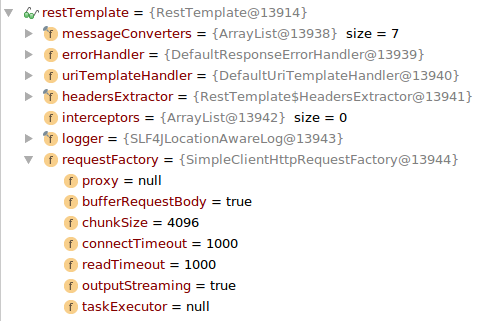
\includegraphics[scale=0.6]{resttempldatedefaulttimeout.png}
	\caption{RestTemplate默认超时时间}
	\label{fig:resttempldatedefaulttimeout}
\end{figure}

上图是Debug跟踪时查看的RestTemplate默认变量。由图中可以看出,默认超时时间是1秒。此时需要增大Read time out的默认超时时间。自定义Read time out超时时间如下代码片段所示:

\begin{lstlisting}[language=Java]
@Bean(name = "commonRestTemplate")
public RestTemplate restTemplate(RestTemplateBuilder restTemplateBuilder) {
	return restTemplateBuilder.setConnectTimeout(5000)
			.setReadTimeout(20000)
			.build();
}
\end{lstlisting}

出现此问题的原因是:当数据量较少时,请求基本能在非常短时间内响应,当数据量逐渐增加时,部分请求处理时间偶尔超过1秒,会出现偶尔失败的情况。

\subsection{自动化部署(Auto Deploy)}

\subsubsection{整体概况}

目前已经将自动化部署应用到部分项目中,省去了非常多手工操作。目前应用的项目情况一览表,表中,CI表示Continuous Integration。

\begin{table}[htbp]
	\caption{自动部署项目信息}
	\label{table:databaseconnectionpool}
	\begin{center}
		\begin{tabular}{|c|c|p{5cm}|}
			\hline
			\multirow{1}{*}{项目名称}
			& \multicolumn{1}{c|}{中文名} 
			& \multicolumn{1}{c|}{说明}\\			
			\cline{1-3}
			report &  通用数据录入子系统  & 通过可灵活调整的配置,动态快速应对不同维度的数据录入场景 \\
			\hline
			report-frontend & 通用数据录入子系统(前端) & 通过可灵活调整的配置,动态快速应对不同维度的数据录入场景,提供动态渲染的,统一的UI \\
			\hline
			system & 主应用 & 主应用 \\
			\hline
			system-frontend & 主应用(前端) & 主应用(前端) \\
			\hline
			system-exchange & 数据交换(exchange)子系统 & 应对所有数据交换场景 \\
			\hline
			system-api & 接口(api)应用 & 接口应用,提供外部数据服务 \\
			\hline
			message & 消息系统 & 站内通知 \\
			\hline
			message-frontend & 消息系统(前端) & 站内通知 \\
			\hline
			web-ci & Web(Continuous Integration) & 网站 \\
			\hline
			web-ci-59 & Web & 网站 \\
			\hline
			web-ci-for-bid & Web & 网站(定制版) \\
			\hline				
		\end{tabular}	
	\end{center}
\end{table}

自动化部署服务器信息如表\ref{table:databaseconnectionpool}所示。提交代码后,构建服务器定时检查代码更新,检查周期可以通过cron表达式定义,若有变更,则触发自动编译构建。应用构建并打包完毕后,会通过调用文件中转服务,将编译完成的应用包拷贝到测试服务器指定目录下。测试服务器上会有定时任务定时调用Shell脚本,Shell脚本会监测应用文件的变化,或者版本定义文件中版本号的变化,任意一项有变动,则触发应用更新。版本变化通过读取版本配置文件来侦测,文件变化通过对比文件的Hash来判断。

\begin{table}[htbp]
	\caption{自动部署服务器信息}
	\label{table:databaseconnectionpool}
	\begin{center}
		\begin{tabular}{|c|c|p{7cm}|}
			\hline
			\multirow{1}{*}{IP}
			& \multicolumn{1}{c|}{名称} 
			& \multicolumn{1}{c|}{备注}\\			
			\cline{1-3}
			192.168.1.24 &  Jenkins服务器  & 所有项目的构建、编译、打包 \\
			\hline
			192.168.1.11 & Nginx服务器 & 文件的接收转发服务 \\
			\hline
			192.168.1.6 & App测试服务器 & 所有App运行在此服务器 \\
			\hline				
		\end{tabular}	
	\end{center}
\end{table}


\subsubsection{构建服务(Auto Build)}

构建服务包含获取源码更新、构建、构建后操作3步。由于项目针对不同应用场景,定义了不同的分支,所以在构建时,需要了解每个分支的含义。各分支定义如表\ref{table:projectbranch}所示:

\begin{table}[htbp]
	\caption{分支名称及含义}
	\label{table:projectbranch}
	\begin{center}
		\begin{tabular}{|c|c|p{5cm}|}
			\hline
			\multirow{1}{*}{项目名称}		 
			& \multicolumn{1}{c|}{分支名称}
			& \multicolumn{1}{c|}{备注}\\			
			\cline{1-3}
			system &  v1.3 & 主分支,1表示第几期,3表示阶段 \\
			\hline
			system & v1.3\_api & 接口分支 \\		
			\hline
			system & v1.3\_exchange & 数据交换分支 \\		
			\hline
			report & develop & 主分支 \\		
			\hline
			report-frontend & develop & 主分支 \\		
			\hline							
		\end{tabular}	
	\end{center}
\end{table}

构建服务定时检查源码仓库的变动,监测到变动后,触发自动编译打包等操作。构建后,通过调用构建后脚本,将文件拷贝到服务器。构建后脚本路径/home/jenkins-bak/,各个脚本的含义如表\ref{table:handlernamingrule}日所示。

\begin{table}[htbp]
	\caption{自动部署后触发脚本命名规则}
	\label{table:handlernamingrule}
	\begin{center}
		\begin{tabular}{|c|p{5cm}|}
			\hline
			\multirow{1}{*}{脚本名称}		 
			& \multicolumn{1}{c|}{备注}\\			
			\cline{1-2}
			\{prject-name\}-after-build-handler.sh &  项目后端构建后处理 \\
			\hline
			\{project-name\}-frontend-after-build-handler.sh  & 项目前端构建后处理 \\		
			\hline				
		\end{tabular}	
	\end{center}
\end{table}

脚本命名含义一般是项目名称加需要产生的作用,project-name表示对应的项目名字,新增时可替换为项目的实际名称。after-build-handler表示此脚本主要告诉Jenkins构建后需要执行此脚本完成一系列动作。构建需要特殊处理的地方:


\begin{lstlisting}[language=Bash]
#!/usr/bin/env bash

# 当使用未初始化的变量时,程序自动退出
set -u

# 当任何一行命令执行失败时,自动退出脚本
set -e

# 在运行结果之前,先输出执行的那一行命令
set -x

readonly APP_ID=""
readonly APP_KEY=""
readonly PROJECT_DIR="/var/lib/jenkins/workspace/web-ci-59"
readonly BUILD_OUTPUT_DIR="/var/lib/jenkins/workspace/web-ci-59/cms/target"

BUILD_DIST_FILENAME=${BUILD_OUTPUT_DIR}/cms.war

cd ${BUILD_OUTPUT_DIR}

#
# 文件过大,无法拷贝
# 将大文件拆分
#
split -b 80M ${BUILD_DIST_FILENAME}

CURRENT_TIME=`date '+%Y-%m-%d %H:%M:%S'`

CONST_STR="ysf"

#
# 生成TOKEN
# 接口各项认证参数的排列顺序是:
# 时间戳(timestamp)、AppKey、随机字符串(echostr)
#
TOKEN=`echo -n ${APP_ID}${APP_KEY}${CURRENT_TIME}${CONST_STR}|md5sum|awk '{print $1}'`
SEQUENCE_TOKEN=`echo -n ${CURRENT_TIME}${APP_ID}${APP_KEY}${CONST_STR}|shasum -a 1|awk '{print $1}'`


# 请求服务端,上传主文件
COMMAND=`curl -H "APPID:$APP_ID" \
-H "TIMESTAMP:$CURRENT_TIME" \
-H "ECHOSTR:$CONST_STR" \
-H "TOKEN:$SEQUENCE_TOKEN" \
-F "file=@${BUILD_OUTPUT_DIR}/xaa" \
http://192.168.1.11:8083/api/fileExchange/upload`

COMMAND=`curl -H "APPID:$APP_ID" \
-H "TIMESTAMP:$CURRENT_TIME" \
-H "ECHOSTR:$CONST_STR" \
-H "TOKEN:$SEQUENCE_TOKEN" \
-F "file=@${BUILD_OUTPUT_DIR}/xab" \
http://192.168.1.11:8083/api/fileExchange/upload`
\end{lstlisting}

在上传文件时,由于限制了文件大小(估计是100MB),当部署文件大于100MB时,使用split命令,拆分成多个小文件分开上传,上传后通过cat命令组装成war包,组装后的文件与原始文件一致,可以通过对比文件的MD5值来判断。

\subsubsection{中转服务(Forward Service)}

中转服务将构建服务器上生成的应用包转发到应用服务器,应用包在测试服务器192.168.1.6的存放路径是/home/deploy/credit。中转服务的配置主要是Nginx转发上传的请求到指定服务器:

\begin{lstlisting}[language=Bash]
location /api/fileExchange {
	proxy_pass http:ip:port;
	proxy_redirect off;
}
\end{lstlisting}

\subsubsection{应用更新服务(Update Trigger)}

应用更新服务在测试服务器,通过建立cron定时任务,轮询检查应用更新情况。定时任务配置文件是/etc/crontab,各个系统更新触发脚本路径是/opt/app/script。定时任务配置示例:

\begin{lstlisting}[language=Bash]
#
# project name update trigger
#
*/1 * * * * root /opt/app/script/project-name-trigger.sh
\end{lstlisting}

触发更新规则在相应的Shell脚本中实现。如下代码片段所示:

\begin{lstlisting}[language=Bash]
#!/usr/bin/env bash

# 部署触发器
# 定时检查文件修改
# 文件修改后,触发部署动作

# 当使用未初始化的变量时,程序自动退出
#set -u

# 当任何一行命令执行失败时,自动退出脚本
set -e

# 在运行结果之前,先输出执行的那一行命令
set -x

# 定义错误日志级别
LOG_LEVEL=-9000

#定义日志存放目录
SIMPLE_LOG_4_SH_DIR=/tmp/simplelog4sh

#导入日志
. /opt/app/script/log4shell.sh

# 当前运行程序版本
readonly APP_PATH="/opt/app/backend-v1.3"
readonly DEPLOY_PATH="/home/deploy/credit"
source ${APP_PATH}/report-version.properties
CURRENT_VERSION=${VERSION}
source ${DEPLOY_PATH}/report-version.properties
DEPLOY_VERSION=${VERSION}
readonly FILE_NAME="report-web-boot-${CURRENT_VERSION}.jar"
readonly DEPLOY_FILE_NAME="report-web-boot-${DEPLOY_VERSION}.jar"

logInfo "检查后端App更新..."

deploy()
{
	logInfo "停止旧版本程序...,版本:${CURRENT_VERSION}"
	ps -ef|grep -w ${FILE_NAME}|grep -v grep|cut -c 9-15|xargs kill 9
	logDebug "开始拷贝新版程序文件....."
	yes|cp -rf ${DEPLOY_PATH}/${DEPLOY_FILE_NAME} ${APP_PATH}
	yes|cp -rf ${DEPLOY_PATH}/credit-report-version.properties ${APP_PATH}
	logInfo "启动新版程序......,程序路径:${APP_PATH},版本:${DEPLOY_VERSION}"
	${APP_PATH}/start-v1.3.sh
}

if test ${CURRENT_VERSION} = ${DEPLOY_VERSION}
then
	logInfo "版本号无变化,检查文件Hash...."
	CURRENT_VERSION_MD5=`md5sum ${APP_PATH}/${FILE_NAME}|cut -d ' ' -f1`
	DEPLOY_VERSION_MD5=`md5sum ${DEPLOY_PATH}/${FILE_NAME}|cut -d ' ' -f1`
	if test ${CURRENT_VERSION_MD5} != ${DEPLOY_VERSION_MD5}
	then
		deploy ""
	else
		logInfo "Hash无变化,文件未修改,后端App结束..."
	fi
else
	logInfo "后端App版本有变化,开始部署新版程序..."
	deploy ""
fi
\end{lstlisting}

由于目前应用较多,单独列出每个应用的目录比较冗长。此处仅仅描述目录的命名的一般性原则。测试环境的目录统一在opt下(项目初始阶段习惯),正式环境的目录在根目录home(初始习惯)或者data下,data目录存放应用是推荐的标准做法,以后新应用部署推荐用此标准,data下存放组织名称对应的目录,组织名称下对应此组织相应的应用。当前各个应用的目录如表\ref{table:projectdirectionayinfo}所示。recommand表示推荐做法,obsolete表示过时的做法,以后不推荐采用的方式。Test表示测试环境,对应的测试服务器IP,Production表示生产环境,对应的生产环境的IP。

\begin{table}[htbp]
	\caption{项目部署目录信息}
	\label{table:projectdirectionayinfo}
	\begin{center}
		\begin{tabular}{|c|c|p{5cm}|c|}
			\hline
			\multirow{1}{*}{IP}
			& \multicolumn{1}{c|}{环境} 
			& \multicolumn{1}{c|}{目录}
			& \multicolumn{1}{c|}{备注}\\			
			\cline{1-4}
			192.168.1.6 &  Test  & /opt/app/ & 部署目录 \\
			\hline
			192.168.1.6 &  Test  & /home/deploy/credit/ & CI部署文件存放目录 \\
			\hline
			192.168.1.6 &  Test  & /opt/app/script/ & CI部署脚本存放目录 \\
			\hline
			10.10.1.* &  Production  & /home/app/ & \textcolor{red}{obsolete} \\
			\hline
			10.10.1.* &  Production  & /data/\{companyname\}/app/ & \textcolor{green}{recommand} \\
			\hline							
		\end{tabular}	
	\end{center}
\end{table}

\subsection{Nginx超时转发}

在后端有双机或多台机器提供服务的情况下,如果某一台机器超过了一定时间未响应,Nginx将尝试将请求转发到下一台服务器。由于写操作时,如果没有在后端作重复校验,一旦写操作比较耗时,转发后会出现重复写的情况(POST一般不进行超时转发,但是幂等请求下也可能会产生重复,比如日志记录、触发消息通知等等)。避免此问题的一种设计方案是在前端渲染表单时,生成一个唯一ID,防止重复提交。所以此处仅仅将超时转发的规则应用在部分url上,在Nginx中的配置如下:

\begin{lstlisting}[language=Bash]
upstream example_upstream{
	server 192.168.0.1 max_fails=1 fail_timeout=3s;
	server 192.168.0.2 max_fails=1 fail_timeout=3s backup;
}
location /example/ {
	proxy_pass http://example_upstream/;
	proxy_set_header Host: test.example.com;
	proxy_set_head X-real-ip $remote_addr;
	proxy_next_upstream error timeout http_500;
}
\end{lstlisting}

Nginx在POST, LOCK, PATCH这种会对服务器造成不幂等的方法,默认是不进行重试的,如果一定要进行重试,则要加上如下配置:

\begin{lstlisting}[language=Bash]
# 非幂等也进行超时转发配置
proxy_next_upstream error timeout http_500 non_idemponent;
\end{lstlisting}

\subsection{无法获取数据库连接}

\begin{quote}
	\textbf{\textcolor{red}{导致问题的原因:数据库连接配置过小,访问量增长时造成连接分配不足,导致无法顺畅访问站点。}}
\end{quote}

最近2天网站运行一段时间后会突然宕掉,日志输出无法获取数据库连接(Could not get JDBC connection),初步推测是数据库连接泄漏,造成数据库可用连接被使用完,主备节点都拿不到连接,造成此问题,目前连接由连接池进行管理,一般情况下是不需要人工干预数据库的连接申请和释放,也有可能是某处进行了手工申请数据库连接,但是没有释放连接导致。使用如下Shell脚本每隔一段时间检测连接池数量:

\begin{lstlisting}[language=Bash]
# 每5秒查看一次到数据库连接个数
nohup watch -n 5 'lsof -i:5236|wc -l >> pool.log'
\end{lstlisting}

经过观察,数据库连接稳定在300-310之间,如果是连接池泄漏,那么连接会随着程序运行逐渐增长,最终达到连接数量上限,根据观察,初步可以排除连接泄漏导致此问题。后来经过日志筛查,发现如下输出:

\begin{lstlisting}[language=Bash]
# 活动连接数
active 20,maxActive 20
\end{lstlisting}

表示当前活动连接数20个,最大活动连接数20个。虽然到数据库的会话有300多个,但是绝大多数是空闲的(Idle),如下语句查看数据库当前会话的个数。

\begin{lstlisting}[language=SQL]
-- 查看数据库当前会话情况
select clnt_ip,state,user_name,count(*)
from v$sessions
group by clnt_ip,state,user_name
\end{lstlisting}

结果如图\ref{fig:sessionstatistics}所示:

\begin{figure}[htbp]
	\centering
	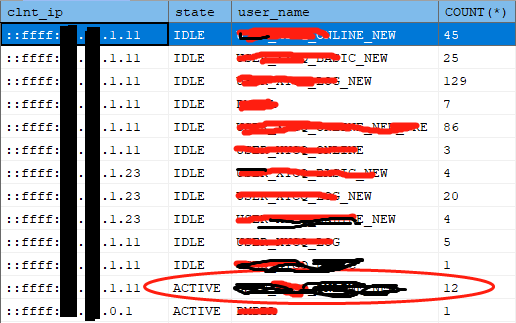
\includegraphics[scale=0.7]{sessionstatistics.png}
	\caption{DB当前连接会话统计}
	\label{fig:sessionstatistics}
\end{figure}

可以看出,活动的会话稳定在13个,离最大个数20已经不远,极有可能是数据库会话配置过小,导致用户增多时,无可用连接分配。为了验证推断,使用JMeter\footnote{\url{http://jmeter.apache.org/}}模拟多用户同时访问测试网站。逐步增加同时访问的用户的个数,当增加到80个时,网站无响应。检查后端日志,出现了线上的问题同样的日志输出,说明问题在此处,需要优化。DBCP当连接数超过最大连接数时,所有连接都会被断开[未找到权威出处]。经过考虑,逐步应用以下优化的方式。

\paragraph{增加网站数据库连接数量上限}调整配置增大数据库连接上限,可以增加网站并发服务能力:

\begin{lstlisting}[language=XML]
<!-- 最小空闲连接数 -->
<property name="minIdle" value="50" />
<!-- 最大连接数 -->
<property name="maxActive" value="100" />
\end{lstlisting}

做了以上优化后,可以提高网站的并发服务量,降低由于访问量过大造成网站不可用的概率,20个连接确实太小,综合评估数据库现有的连接资源(500),调整后连接数分配情况:

\begin{table}[htbp]
	\caption{应用连接个数分配情况}
	\label{table:projectdirectionayinfo}
	\begin{center}
		\begin{tabular}{|c|c|p{2cm}|}
			\hline
			\multirow{1}{*}{环境}
			& \multicolumn{1}{c|}{IP} 
			& \multicolumn{1}{c|}{连接个数}\\			
			\cline{1-3}
			主机 &  192.168.1.1  & 100 \\
			\hline
			备机 &  192.168.1.23  & 100 \\
			\hline
			移动端 &  192.168.1.1  & 100 \\
			\hline
			旧版App、定制版App、登陆、临时使用预留 &  192.168.1.*  & 200 \\
			\hline									
		\end{tabular}	
	\end{center}
\end{table}

\paragraph{增大数据库Session数量上限}目前数据库的会话数量是500,可以调整为1000。

\paragraph{缓存页面信息}实际上,页面在绝大部分时间是不会改变的,完全可以将页面信息缓存在Redis中,不但减轻数据库压力,还可成倍提高网站响应速度和并发处理能力。此种优化方式需要对代码做一定程度改造,比如发布信息时,需要清除对应模块的Redis缓存信息,保证信息更新及时。

\paragraph{将流量分配到不同的机器}后端流量可以主备机同时启用,涉及到Session共享问题,需要进一步测试。

\section{编辑中}

\subsection{内存溢出异常}

上周网站Down掉,本周接口Down掉,愉快的周末泡汤了。所以,暗自忖度,一定要找到问所在。内存溢出一般分为2种情况,一时是超出预期的访问量/数据量,另一种是内存泄露(Memory leak)。第一次的内存溢出异常有hprof文件,将文件拷贝出来进行分析。第二次接口异常没有生成hprof,采用VisualVM分析内存情况。在服务端启动jstatd(Java State Daemon)守护进程:

\begin{lstlisting}[language=Bash]
# 
./jstatd -J-Djava.security.policy=../jstatd.all.policy -J-Djava.rmi.server.hostname=10.10.1.53
jmap -dump:format=b,file=/opt [pid]
\end{lstlisting}

在本地使用VisualVM监视服务端JVM的运行情况,内存的增长速度在4-5MB/s,2GB的内存在4-5min就被消耗完毕,接着进行一次YGC(Young Garbage Collection)。



\subsection{XX-Net}










\begin{thebibliography}{0}
\bibitem{蒋金楠MVC框架揭秘}
蒋金楠.《ASP.NET MVC 5框架揭秘》.电子工业出版社,2014.
\end{thebibliography}

%\bibitem{BSD}
%B. Birch, H. P. F. Swinnerton-Dyer, \emph{Notes on ellptic curves (II)}. J Reine Angrew Math, 1965, 218:79-108.
\end{document}
